\documentclass[11pt]{report}

% ==================== Imports ====================
\usepackage[margin=1in]{geometry}
\usepackage{graphicx}
\usepackage{amssymb} % required for \checkmark used in the roles table
\usepackage{tikz}
\usetikzlibrary{shapes.geometric,shapes.multipart,arrows.meta,positioning,calc,fit,backgrounds,decorations.pathreplacing}
\usepackage{pgf-umlcd}
\usepackage{booktabs}
\usepackage{array}
\usepackage{tabularx}
\usepackage{longtable}
\usepackage{enumitem}
\setlist{itemsep=2pt, topsep=3pt, parsep=0pt}
\usepackage{xcolor}
\usepackage{caption}
\usepackage{float}
\usepackage{xspace}
\usepackage{hyperref}

\newcommand{\sysname}{Civic Issue Reporter\xspace}

\begin{document}
\raggedbottom

% ==================== Title Page (manually built, no custom class needed) ====================
\begin{titlepage}
  \centering
  \large UCS503P - Software Engineering Project\par
  \vspace{2cm}
  {\Huge\bfseries Civic Issue Reporter\par}
  \vspace{0.8cm}
  {\large A Role-Based Web Platform for Reporting, Routing, and Resolving\\
  Campus Infrastructure Issues at TIET\par}
  \vspace{2cm}
  \begin{tabular}{l}
    \texttt{1024030227} Lavanya Sharma \\
    \texttt{1024030309} Parismita Thapa \\
    \texttt{1024030389} Rudra Yadav \\
    \texttt{1024030291} Nadeem Esrar
  \end{tabular}
  \vspace{1.5cm}

  \large BE Third Year, Computer Engineering (COE)\par
  \vspace{1cm}
  Advisor: Ms.\ Anushka\par
  \vfill
  {\large Mid-Semester Evaluation\par}
  \vspace{0.2cm}
  \textbf{Computer Science and Engineering Department}\par
  \vspace{0.15cm}
  Thapar Institute of Engineering and Technology, Patiala\par
\end{titlepage}

\tableofcontents

% ===================================================================
% CHAPTER 1: INTRODUCTION
% ===================================================================
\chapter{Introduction}

\section{Background and Context}

Campus infrastructure faults at the Thapar Institute of Engineering and
Technology (TIET) -- broken equipment, plumbing leaks, faulty wiring,
damaged furniture, non-functional washrooms, and unsafe walkways -- are
today reported informally: through hostel WhatsApp groups, verbal
complaints to wardens, or ad-hoc emails to department staff. TIET's
campus spans multiple hostels, academic blocks, and shared facilities
(the library, cafeterias, the sports complex) maintained by different
departments. Because the reporting channel is informal and
department-specific, the effective bottleneck in resolving these issues
is not maintenance capacity itself but \emph{issue visibility and
routing}: nobody has a shared, authoritative view of what has already
been reported, to whom, and at what stage it stands.

The \sysname project applies standard software engineering
practice~\cite{sommerville2016} -- requirement analysis, system design,
and structured, iterative development -- to this real campus problem. The broader
motivation is to improve campus infrastructure governance by reducing
the time and effort required to resolve civic issues reported by
students and faculty. The immediate engineering objective is to design
and implement a measurable, deployable web platform for efficient,
department-routed issue resolution across academic blocks, hostels, the
library, cafeterias, the sports complex, and other common areas.

\subsection{Problem Statement}

The absence of a structured reporting channel produces several concrete
problems:

\begin{itemize}
  \item \textbf{No single source of truth:} the same issue is reported
    independently to multiple people, with no shared record of what has
    already been flagged or fixed.
  \item \textbf{No accountability or tracking:} a reporter has no way to
    check whether a complaint was received, let alone what stage it is
    at.
  \item \textbf{No severity-aware prioritization:} a loose wire in a
    washroom and a broken chair in a common room compete for the same
    informal attention, with no structural way to surface
    safety-critical issues first.
  \item \textbf{Redundant effort:} without a shared, searchable list of
    open issues, students and faculty re-report problems that are
    already known, and administrators re-investigate what has already
    been logged.
  \item \textbf{No institutional visibility:} there is no aggregate view
    -- by building, department, or category -- that lets facilities
    management identify recurring or high-impact problem areas.
\end{itemize}

\section{Project Objectives}

The primary goal of the project is to design and deploy a role-based web
platform that gives the TIET campus community a structured, trackable
channel for reporting and resolving infrastructure issues, while
reducing duplicate reporting and improving response time to
high-priority faults. This goal is decomposed into the following SMART
(Specific, Measurable, Achievable, Relevant, Time-bound) objectives:

\begin{enumerate}
  \item \textbf{Objective 1 -- Low-friction reporting:} Give students
    and faculty a single channel to report infrastructure issues with a
    photo, category, and precise structured location, deliverable as a
    working submission form by Week 4 of the project timeline.
  \item \textbf{Objective 2 -- Automatic, correctable routing:}
    Automatically route each report to the right department using a
    category-to-department mapping, while still allowing a manual
    override when the auto-suggested category is wrong, deliverable
    alongside the submission flow.
  \item \textbf{Objective 3 -- Duplicate prevention:} Prevent duplicate
    reports of the same problem from fragmenting attention by detecting
    likely duplicates at submission time (location, department, and
    description-similarity signals) and letting users upvote an
    existing report instead, targeted for Weeks 5--6.
  \item \textbf{Objective 4 -- Priority-aware escalation:} Ensure
    high-impact or safety-critical issues are not left to languish in a
    queue by automatically escalating priority once an issue's upvote
    count crosses a configurable threshold, targeted for Week 9.
  \item \textbf{Objective 5 -- Closed feedback loop:} Close the feedback
    loop for reporters through status-change and escalation
    notifications, so that ``I reported it and heard nothing'' is no
    longer the default experience.
  \item \textbf{Objective 6 -- Scoped administrative control:} Give
    department Administrators and a Super-Admin department-scoped and
    institution-wide visibility respectively, so ownership of an issue
    is always clear.
\end{enumerate}

% ===================================================================
% CHAPTER 2: METHODOLOGY AND DESIGN
% ===================================================================
\chapter{Methodology and Design}

\section{System Architecture}

\subsection{High-Level Design}

The \sysname is designed as a three-tier web application (see
Figure~\ref{fig:architecture}). A React single-page frontend serves two
distinct experiences from the same codebase: a low-friction submission
and browsing view for students/faculty, and a status-management
dashboard for Administrators and the Super-Admin. All client requests
pass through a stateless REST API~\cite{fielding2000rest} built on
Node.js/Express, which is
responsible for authentication and role-based access control (RBAC),
issue submission and department routing, the duplicate-detection
heuristic, the auto-escalation check, and notification generation. The
API persists relational data -- issues, users, departments, upvotes, and
notifications -- in a managed PostgreSQL instance~\cite{postgresql2024},
while photo
attachments are stored separately in object storage (Cloudinary/AWS S3)
so that image growth does not pressure the primary database. A CI/CD
pipeline (GitHub Actions) builds, lints, and tests the backend on every
change and deploys to a staging environment, in line with the project's
weekly iteration cadence.

\begin{figure}[H]
  \centering
  \resizebox{\textwidth}{!}{%
  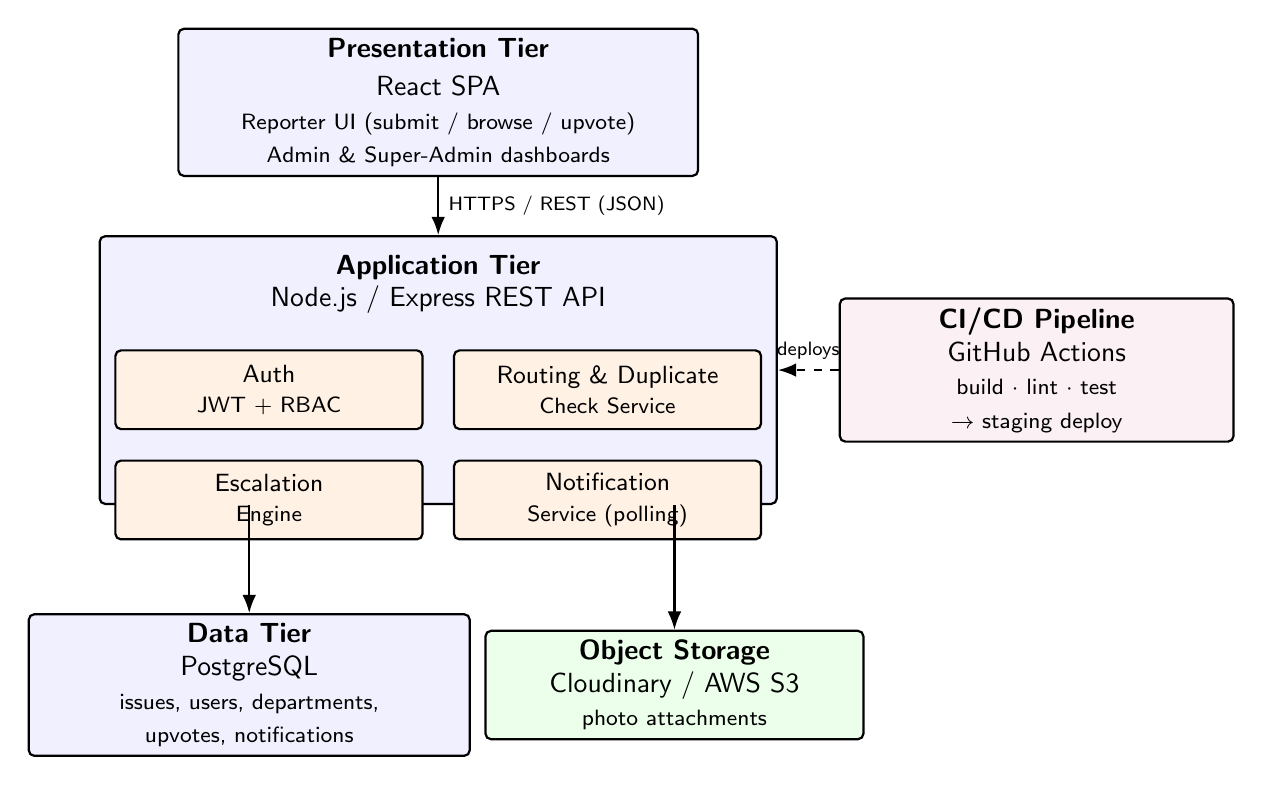
\begin{tikzpicture}[
      box/.style={draw, thick, rounded corners=2pt, minimum height=1.1cm,
        align=center, fill=blue!6, font=\sffamily},
      infra/.style={draw, thick, rounded corners=2pt, minimum height=1cm,
        align=center, fill=orange!10, font=\sffamily\small},
      arrowstyle/.style={-Latex, thick},
      every node/.style={font=\sffamily}
    ]
    % Tier 1: Client
    \node[box, minimum width=6.6cm] (client) at (0,6)
      {\textbf{Presentation Tier}\\[2pt]
       React SPA\\
       \footnotesize Reporter UI (submit / browse / upvote)\\
       \footnotesize Admin \& Super-Admin dashboards};

    % Tier 2: API
    \node[box, minimum width=8.6cm, minimum height=3.4cm] (api) at (0,2.6)
      {};
    \node[align=center, font=\sffamily\bfseries] at (0,3.9) {Application Tier};
    \node[align=center, font=\sffamily] at (0,3.5) {Node.js / Express REST API};
    \node[infra, minimum width=3.9cm] (auth) at (-2.15,2.35) {Auth \\ \footnotesize JWT + RBAC};
    \node[infra, minimum width=3.9cm] (route) at (2.15,2.35) {Routing \& Duplicate\\\footnotesize Check Service};
    \node[infra, minimum width=3.9cm] (esc) at (-2.15,0.95) {Escalation\\\footnotesize Engine};
    \node[infra, minimum width=3.9cm] (notif) at (2.15,0.95) {Notification\\\footnotesize Service (polling)};

    % Tier 3: Data
    \node[box, minimum width=5.6cm] (db) at (-2.4,-1.4)
      {\textbf{Data Tier}\\ PostgreSQL\\ \footnotesize issues, users, departments,\\ \footnotesize upvotes, notifications};

    % Object storage
    \node[box, minimum width=4.8cm, fill=green!8] (store) at (3,-1.4)
      {\textbf{Object Storage}\\ Cloudinary / AWS S3\\ \footnotesize photo attachments};

    % CI/CD
    \node[box, minimum width=5.0cm, fill=purple!6] (cicd) at (7.6,2.6)
      {\textbf{CI/CD Pipeline}\\ GitHub Actions\\ \footnotesize build $\cdot$ lint $\cdot$ test\\ \footnotesize $\rightarrow$ staging deploy};

    % Arrows
    \draw[arrowstyle] (client) -- node[right, font=\scriptsize\sffamily]{HTTPS / REST (JSON)} (api.north);
    \draw[arrowstyle] (api.south -| db.north) -- (db.north);
    \draw[arrowstyle] (api.south -| store.north) -- (store.north);
    \draw[arrowstyle, dashed] (cicd) -- node[above, font=\scriptsize\sffamily]{deploys} (api.east);
  \end{tikzpicture}}
  \caption{Three-tier system architecture of the Civic Issue Reporter platform.}
  \label{fig:architecture}
\end{figure}

\subsection{Use Case View}

Figure~\ref{fig:usecase} presents the system's use-case model. Students
and Faculty are modelled as functionally identical actors: both may
report an issue (which includes a duplicate check), view the full list
of reported issues read-only, and upvote an existing issue instead of
filing a new one. An Administrator can view and update the status of
issues owned by their own department, while the Super-Admin
generalizes an Administrator and additionally oversees issues across
\emph{all} departments.

\begin{figure}[H]
  \centering
  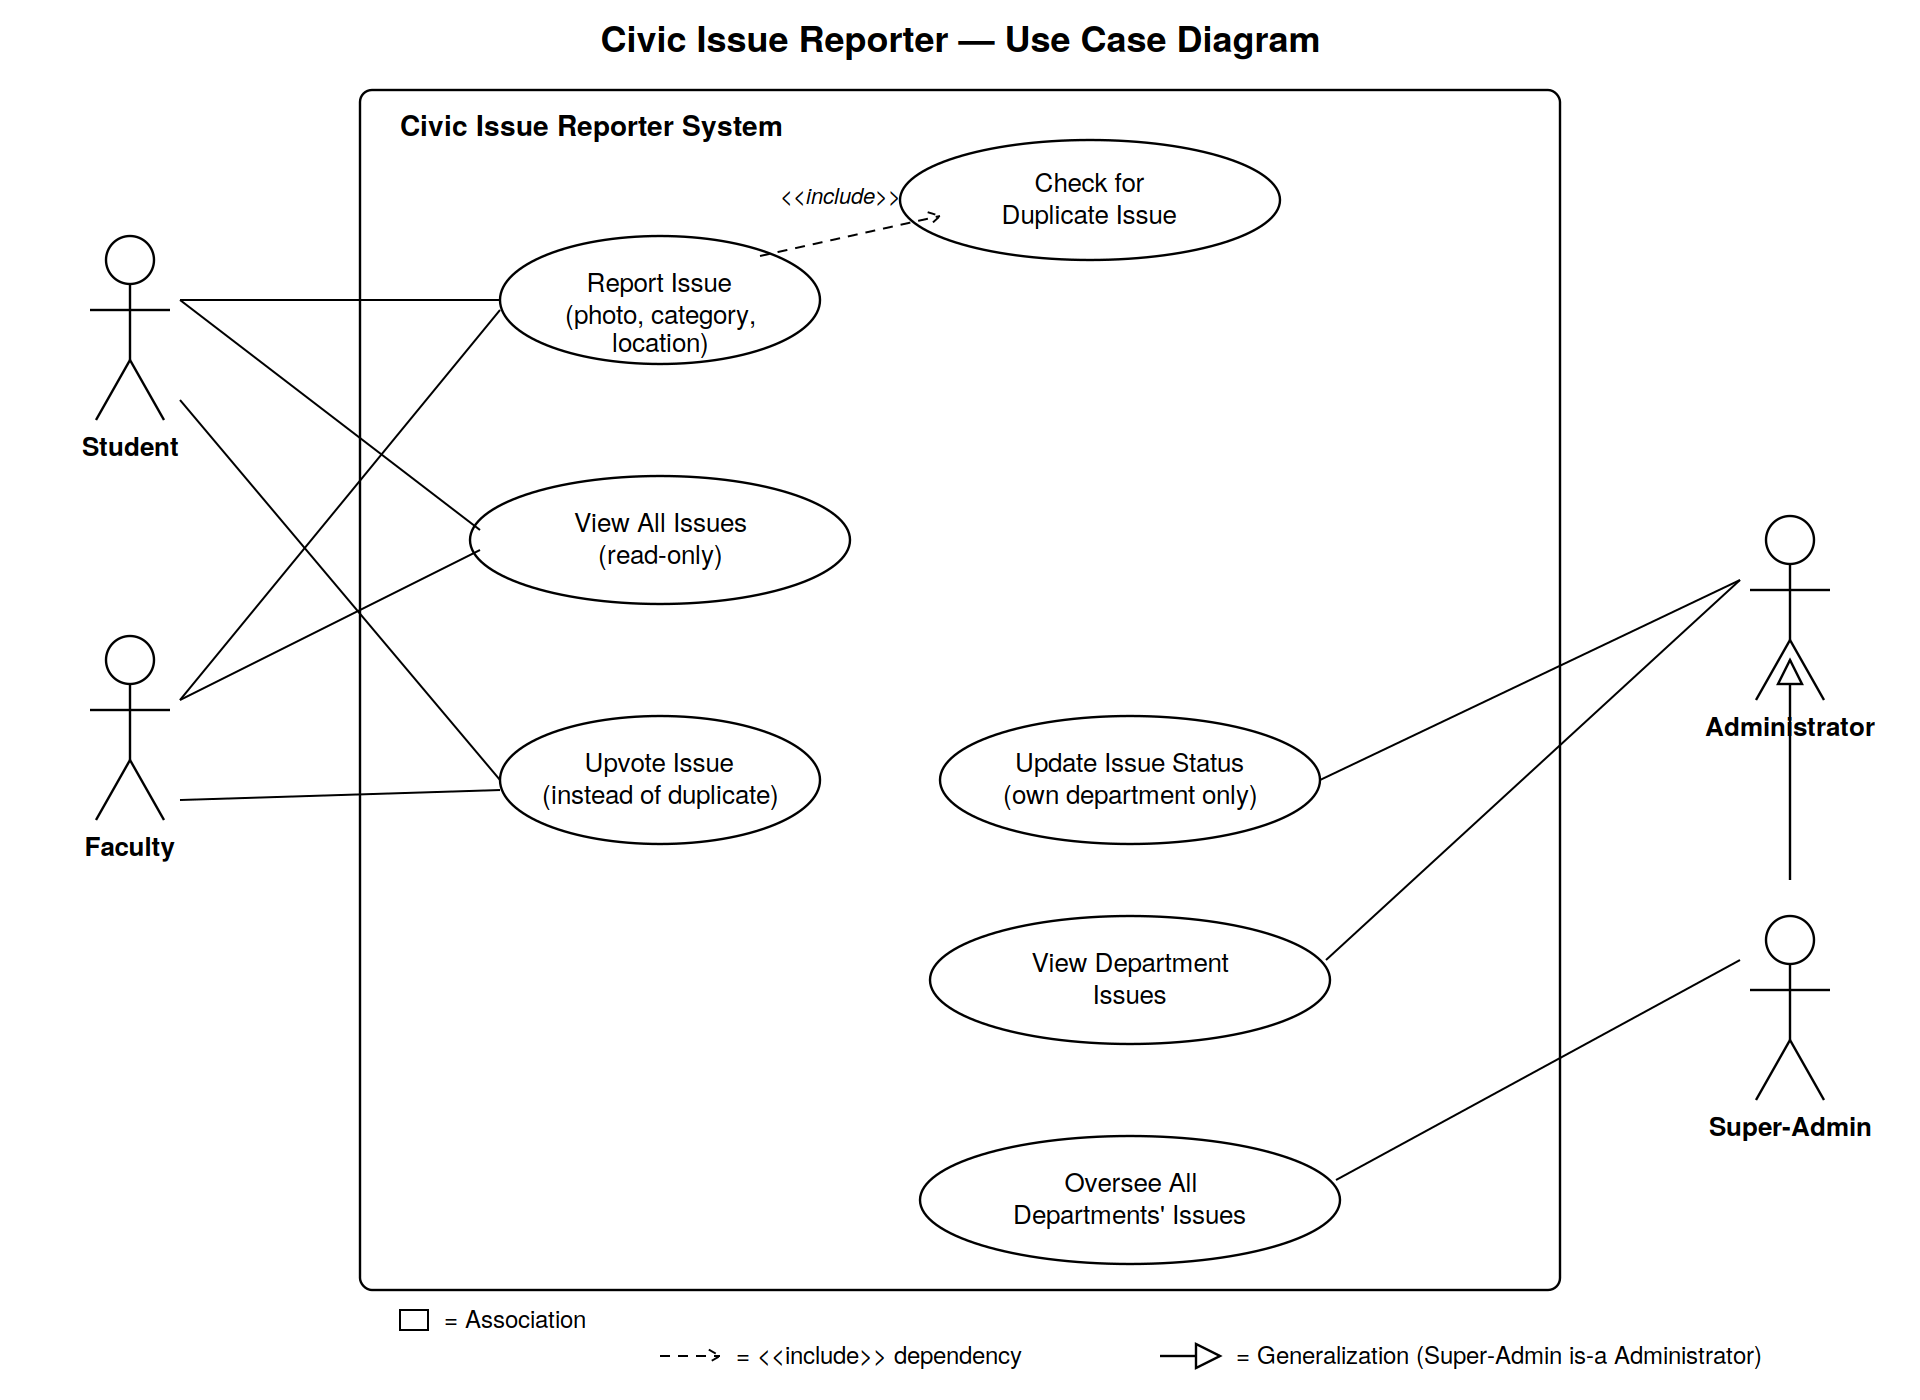
\includegraphics[width=0.95\textwidth]{use_case_diagram.png}
  \caption{Use case diagram for the Civic Issue Reporter system.}
  \label{fig:usecase}
\end{figure}

\subsection{Technical Stack}

\begin{table}[H]
\centering
\begin{tabular}{|p{2.6cm}|p{3.6cm}|p{8cm}|}
\hline
\textbf{Tier} & \textbf{Technology} & \textbf{Purpose} \\
\hline
Frontend & React & Responsive UI for reporters (submission form, status view) and administrators (dashboard), usable on low-to-mid range student devices. \\
\hline
Backend API & Node.js / Express (Flask fallback) & REST API for authentication, submission, routing, status transitions, and escalation logic. \\
\hline
Database & PostgreSQL & Maintains relational integrity between issues, departments, users, upvotes, and notifications; indexed on location, department, and status for duplicate detection and dashboards. \\
\hline
Object storage & Cloudinary / AWS S3 & Stores photo attachments outside the primary database. \\
\hline
Auth & JWT + RBAC & Stateless session tokens with role-based access enforced at the API layer for all four roles. \\
\hline
CI/CD & GitHub Actions & Build, lint, and test on every change; deploy to staging. \\
\hline
\end{tabular}
\caption{Technology choices by architectural tier.}
\label{tab:web-architecture}
\end{table}

\section{Data Model}

Figure~\ref{fig:classdiagram} shows the core class/data model, drawn
using standard UML class-diagram notation~\cite{fowler2004uml} and
informed by relational data-modelling practice~\cite{elmasri2015}.
\texttt{User}
is specialised into \texttt{Student}, \texttt{Faculty}, and
\texttt{Administrator}, with \texttt{SuperAdmin} further specialising
\texttt{Administrator} -- reflecting that a Super-Admin is a superset of
an Administrator's capabilities plus cross-department oversight. Every
\texttt{Issue} belongs to exactly one \texttt{Department} and may
receive many \texttt{Upvote} records, each tied to exactly one
\texttt{User}; a unique constraint on the (\texttt{userId},
\texttt{issueId}) pair on \texttt{Upvote} prevents a single user from
inflating an issue's count. \texttt{Notification} records the four
event types described in Section~\ref{sec:notifications} and are always
addressed to a single \texttt{User}.

\begin{figure}[H]
  \centering
  \resizebox{\textwidth}{!}{%
  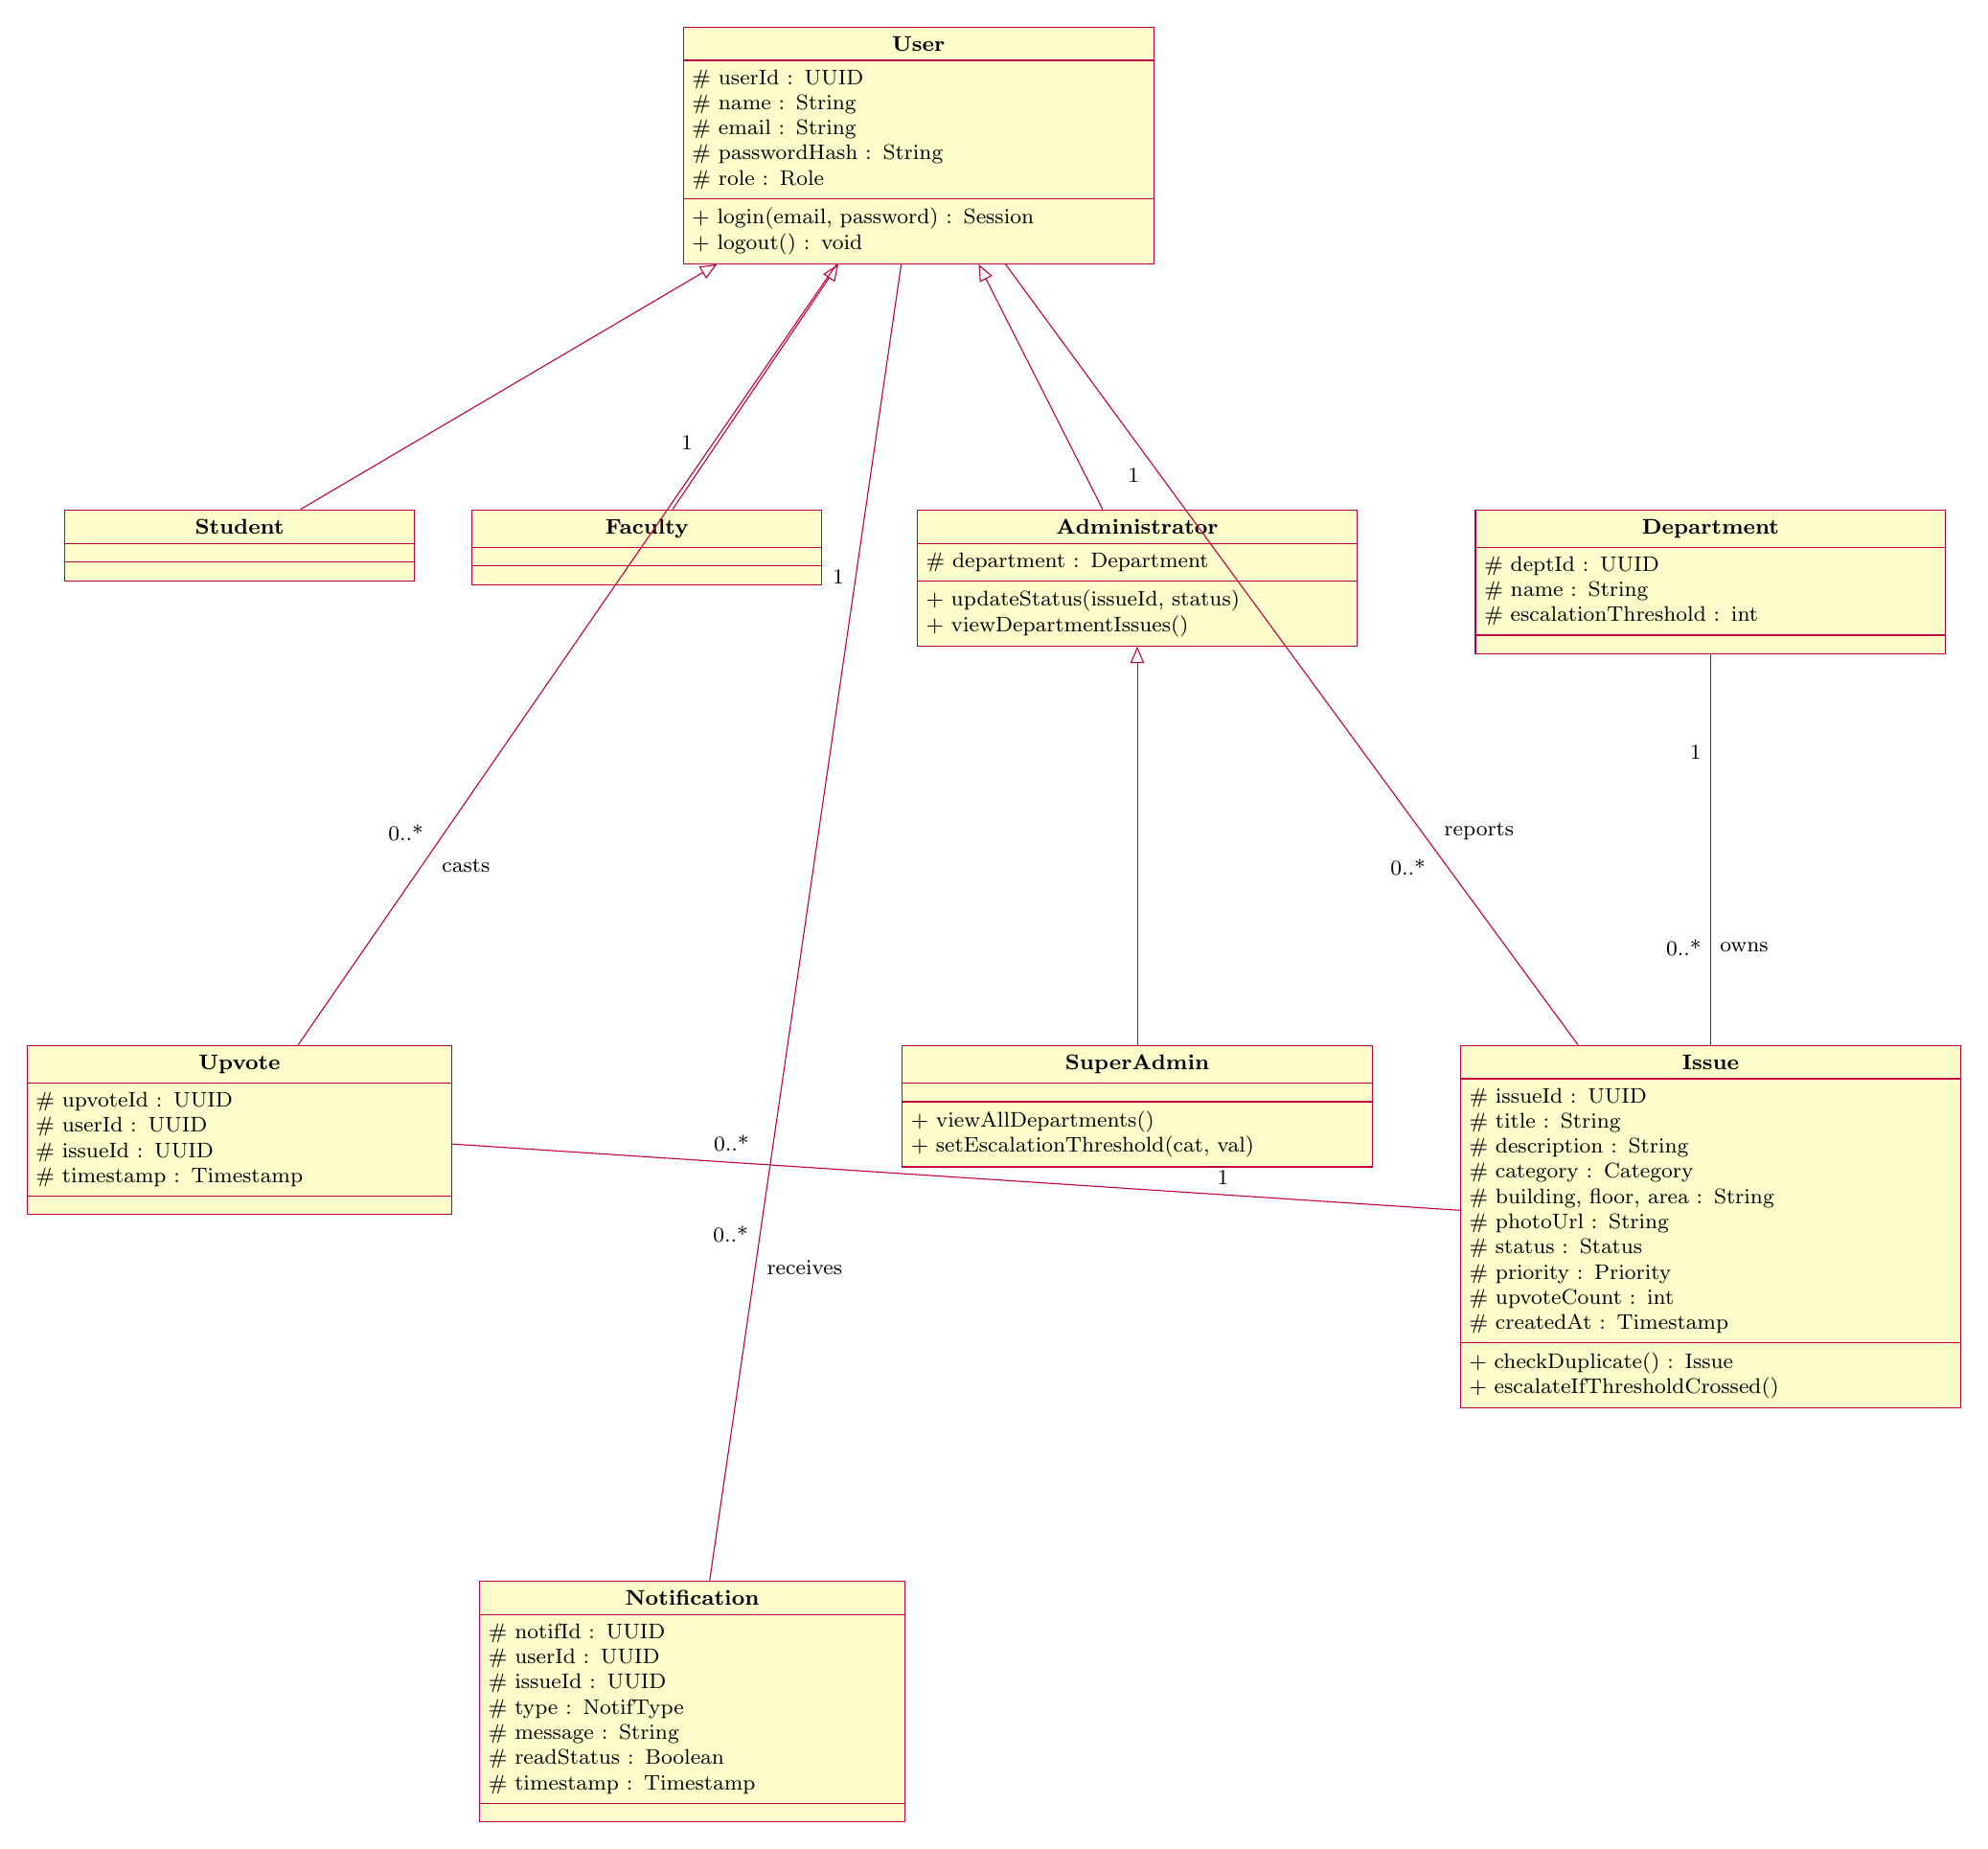
\begin{tikzpicture}[font=\footnotesize]

  \begin{class}[text width=6cm]{User}{0,14}
    \attribute{\# userId : UUID}
    \attribute{\# name : String}
    \attribute{\# email : String}
    \attribute{\# passwordHash : String}
    \attribute{\# role : Role}
    \operation{+ login(email, password) : Session}
    \operation{+ logout() : void}
  \end{class}

  \begin{class}[text width=4.4cm]{Student}{-9,7.6}
    \inherit{User}
  \end{class}

  \begin{class}[text width=4.4cm]{Faculty}{-3.6,7.6}
    \inherit{User}
  \end{class}

  \begin{class}[text width=5.6cm]{Administrator}{2.9,7.6}
    \attribute{\# department : Department}
    \operation{+ updateStatus(issueId, status)}
    \operation{+ viewDepartmentIssues()}
    \inherit{User}
  \end{class}

  \begin{class}[text width=6cm]{SuperAdmin}{2.9,0.5}
    \operation{+ viewAllDepartments()}
    \operation{+ setEscalationThreshold(cat, val)}
    \inherit{Administrator}
  \end{class}

  \begin{class}[text width=6cm]{Department}{10.5,7.6}
    \attribute{\# deptId : UUID}
    \attribute{\# name : String}
    \attribute{\# escalationThreshold : int}
  \end{class}

  \begin{class}[text width=6.4cm]{Issue}{10.5,0.5}
    \attribute{\# issueId : UUID}
    \attribute{\# title : String}
    \attribute{\# description : String}
    \attribute{\# category : Category}
    \attribute{\# building, floor, area : String}
    \attribute{\# photoUrl : String}
    \attribute{\# status : Status}
    \attribute{\# priority : Priority}
    \attribute{\# upvoteCount : int}
    \attribute{\# createdAt : Timestamp}
    \operation{+ checkDuplicate() : Issue}
    \operation{+ escalateIfThresholdCrossed()}
  \end{class}

  \begin{class}[text width=5.4cm]{Upvote}{-9,0.5}
    \attribute{\# upvoteId : UUID}
    \attribute{\# userId : UUID}
    \attribute{\# issueId : UUID}
    \attribute{\# timestamp : Timestamp}
  \end{class}

  \begin{class}[text width=5.4cm]{Notification}{-3,-6.6}
    \attribute{\# notifId : UUID}
    \attribute{\# userId : UUID}
    \attribute{\# issueId : UUID}
    \attribute{\# type : NotifType}
    \attribute{\# message : String}
    \attribute{\# readStatus : Boolean}
    \attribute{\# timestamp : Timestamp}
  \end{class}

  \association{User}{}{1}{Issue}{reports}{0..*}
  \association{User}{}{1}{Upvote}{casts}{0..*}
  \association{Issue}{}{1}{Upvote}{}{0..*}
  \association{Department}{}{1}{Issue}{owns}{0..*}
  \association{User}{}{1}{Notification}{receives}{0..*}

  \end{tikzpicture}}
  \caption{Class diagram / core data model of the Civic Issue Reporter system.}
  \label{fig:classdiagram}
\end{figure}

\section{Process Model}

\subsection{Context and Level-1 Data Flow Diagrams}

Figures~\ref{fig:dfd0} and~\ref{fig:dfd1} present the Gane--Sarson data
flow diagrams for the system. The Context Diagram (Level 0) fixes the
system boundary and its external entities -- Student/Faculty,
Administrator, and Super-Admin -- and the major information flows
between them and the system. The Level-1 diagram decomposes the system
into its major processes (submission and duplicate check, routing,
status update, and escalation/notification) and the data stores they
read from or write to.

\begin{figure}[H]
  \centering
  \resizebox{0.85\textwidth}{!}{%
  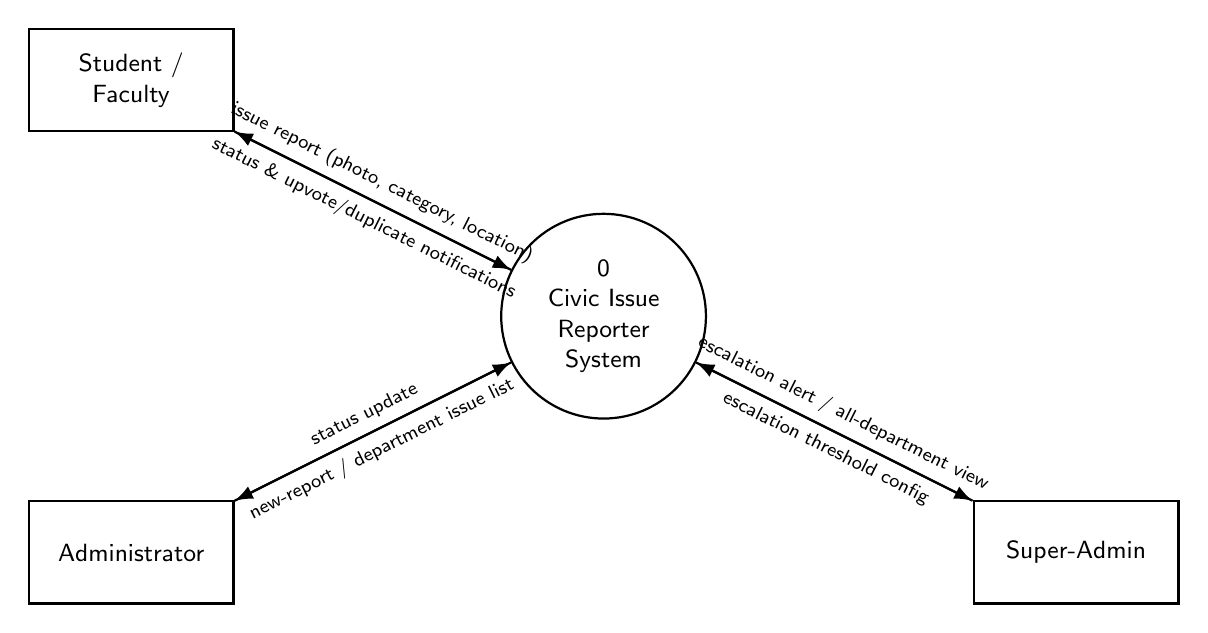
\begin{tikzpicture}[
      entity/.style={draw, thick, minimum width=2.6cm, minimum height=1.3cm, align=center, font=\sffamily\small},
      process/.style={draw, thick, circle, minimum size=2.6cm, align=center, font=\sffamily\small},
      arrowstyle/.style={-Latex, thick, font=\scriptsize\sffamily}
    ]
    \node[entity] (student) at (-6,3) {Student /\\Faculty};
    \node[entity] (admin) at (-6,-3) {Administrator};
    \node[entity] (super) at (6,-3) {Super-Admin};
    \node[process] (sys) at (0,0) {0\\Civic Issue\\Reporter\\System};

    \draw[arrowstyle] (student) -- node[above, sloped]{issue report (photo, category, location)} (sys);
    \draw[arrowstyle] (sys) -- node[below, sloped]{status \& upvote/duplicate notifications} (student);
    \draw[arrowstyle] (admin) -- node[above, sloped]{status update} (sys);
    \draw[arrowstyle] (sys) -- node[below, sloped]{new-report / department issue list} (admin);
    \draw[arrowstyle] (sys) -- node[above, sloped]{escalation alert / all-department view} (super);
    \draw[arrowstyle] (super) -- node[below, sloped]{escalation threshold config} (sys);
  \end{tikzpicture}}
  \caption{Context (Level 0) data flow diagram.}
  \label{fig:dfd0}
\end{figure}

\begin{figure}[H]
  \centering
  \resizebox{\textwidth}{!}{%
  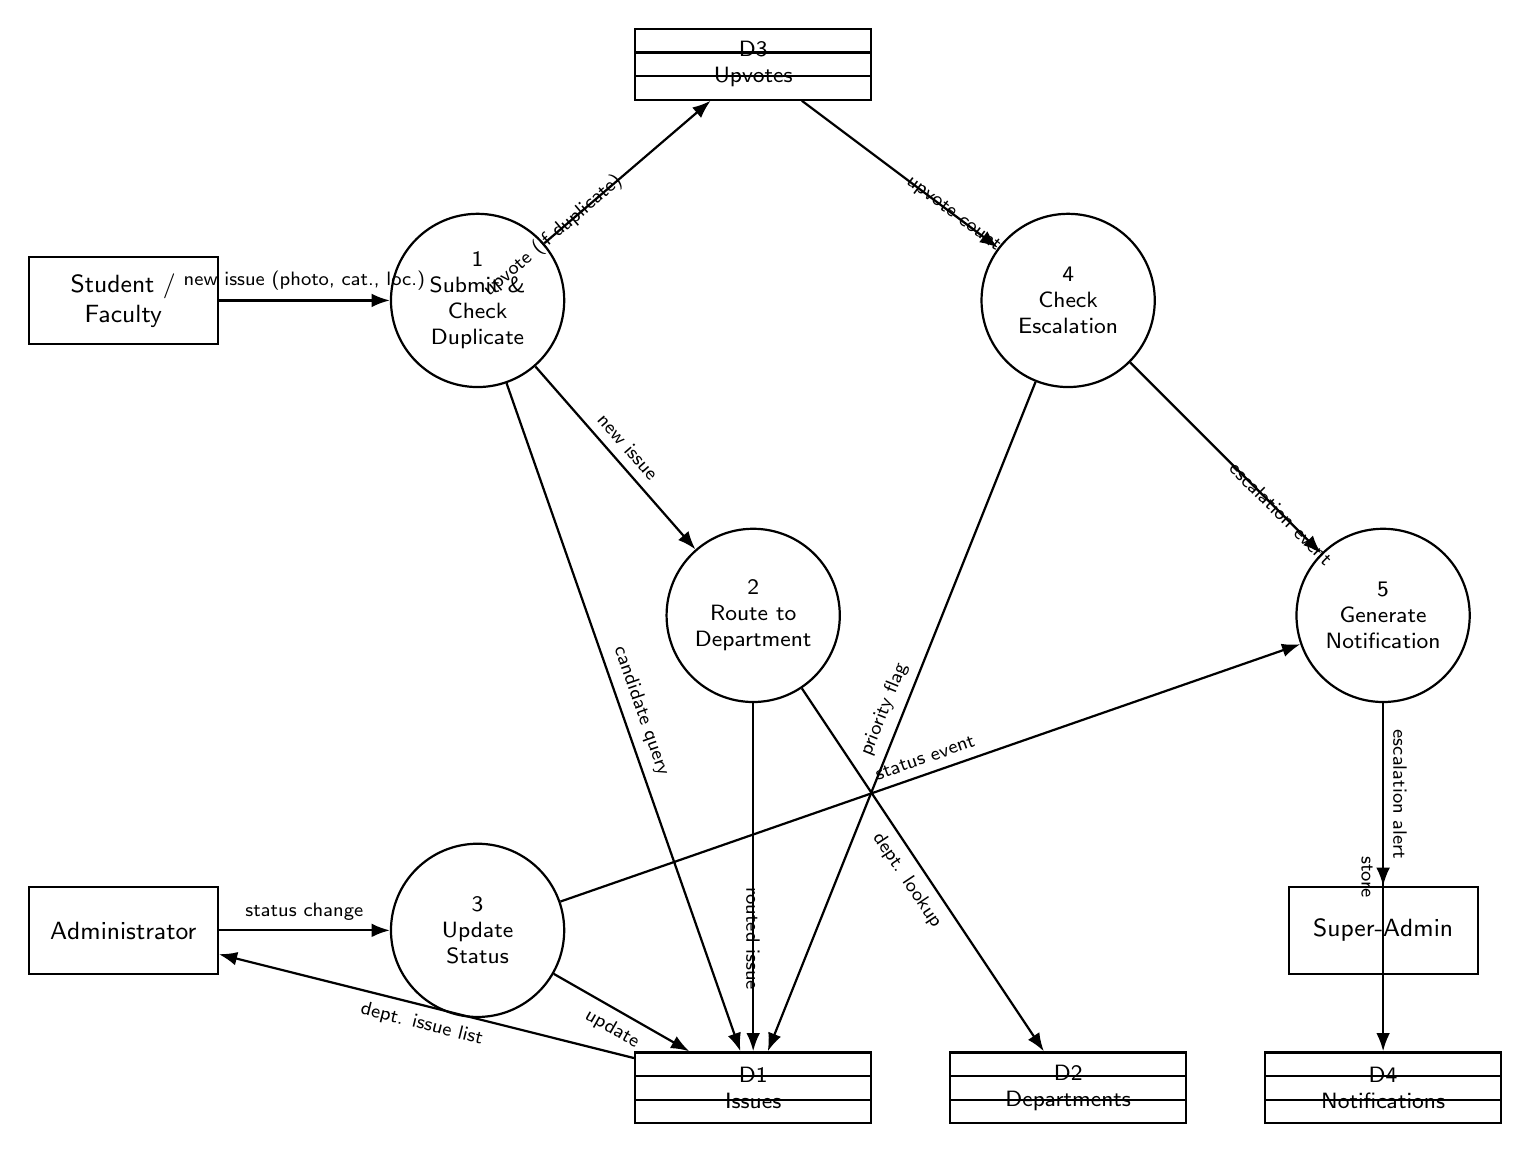
\begin{tikzpicture}[
      entity/.style={draw, thick, minimum width=2.4cm, minimum height=1.1cm, align=center, font=\sffamily\small},
      process/.style={draw, thick, circle, minimum size=2.2cm, align=center, font=\sffamily\footnotesize},
      store/.style={draw, thick, minimum width=3cm, minimum height=0.9cm, align=center, font=\sffamily\footnotesize, path picture={
        \draw ([yshift=-0.3cm]path picture bounding box.north west) -- ([yshift=-0.3cm]path picture bounding box.north east);
        \draw ([yshift=0.3cm]path picture bounding box.south west) -- ([yshift=0.3cm]path picture bounding box.south east);
      }},
      arrowstyle/.style={-Latex, thick, font=\scriptsize\sffamily}
    ]
    \node[entity] (reporter) at (-8,4) {Student /\\Faculty};
    \node[entity] (admin) at (-8,-4) {Administrator};
    \node[entity] (super) at (8,-4) {Super-Admin};

    \node[process] (p1) at (-3.5,4) {1\\Submit \&\\Check\\Duplicate};
    \node[process] (p2) at (0,0)   {2\\Route to\\Department};
    \node[process] (p3) at (-3.5,-4) {3\\Update\\Status};
    \node[process] (p4) at (4,4)  {4\\Check\\Escalation};
    \node[process] (p5) at (8,0)  {5\\Generate\\Notification};

    \node[store] (d1) at (0,-6) {D1 \\ Issues};
    \node[store] (d2) at (4,-6) {D2 \\ Departments};
    \node[store] (d3) at (0,7)  {D3 \\ Upvotes};
    \node[store] (d4) at (8,-6) {D4 \\ Notifications};

    \draw[arrowstyle] (reporter) -- node[above,sloped]{new issue (photo, cat., loc.)} (p1);
    \draw[arrowstyle] (p1) -- node[above,sloped]{candidate query} (d1);
    \draw[arrowstyle] (p1) -- node[left,sloped]{upvote (if duplicate)} (d3);
    \draw[arrowstyle] (p1) -- node[above,sloped]{new issue} (p2);
    \draw[arrowstyle] (p2) -- node[below,sloped]{dept. lookup} (d2);
    \draw[arrowstyle] (p2) -- node[right,sloped]{routed issue} (d1);
    \draw[arrowstyle] (admin) -- node[above,sloped]{status change} (p3);
    \draw[arrowstyle] (p3) -- node[below,sloped]{update} (d1);
    \draw[arrowstyle] (d3) -- node[right,sloped]{upvote count} (p4);
    \draw[arrowstyle] (p4) -- node[above,sloped]{priority flag} (d1);
    \draw[arrowstyle] (p3) -- node[above,sloped]{status event} (p5);
    \draw[arrowstyle] (p4) -- node[right,sloped]{escalation event} (p5);
    \draw[arrowstyle] (p5) -- node[below,sloped]{store} (d4);
    \draw[arrowstyle] (p5) -- node[above,sloped]{escalation alert} (super);
    \draw[arrowstyle] (d1) -- node[below,sloped]{dept. issue list} (admin);
  \end{tikzpicture}}
  \caption{Level-1 data flow diagram decomposing the system's major processes.}
  \label{fig:dfd1}
\end{figure}

\subsection{Core Workflow}
\label{sec:notifications}

Figure~\ref{fig:activity} models the end-to-end reporting workflow as a
UML activity diagram. A student or faculty member submits an issue with
a photo, category, and structured location. The system auto-suggests a
department and, in the same step, checks for likely duplicates among
\emph{open} issues in that location/department bucket. If a likely
duplicate is found, the reporter is shown it and may upvote it instead
of creating a new record; otherwise a new issue is created in
\texttt{Reported} status and routed to the relevant Administrator, who
is notified. As upvotes accumulate, the system checks the issue's count
against its category's escalation threshold on every upvote event; on
crossing it, the issue is marked \emph{High Priority} and the
Super-Admin is notified. The owning Administrator (or Super-Admin)
subsequently moves the issue through \texttt{Reported}
$\rightarrow$ \texttt{Ongoing} $\rightarrow$ \texttt{Finished}; the
original reporter is notified at each transition. Four notification
types are generated across this workflow: status-change (to the
reporter), upvote/duplicate activity (to the reporter), new-report
(to the owning department's Administrator), and escalation (to the
Super-Admin).

\begin{figure}[H]
  \centering
  \resizebox{0.8\textwidth}{!}{%
  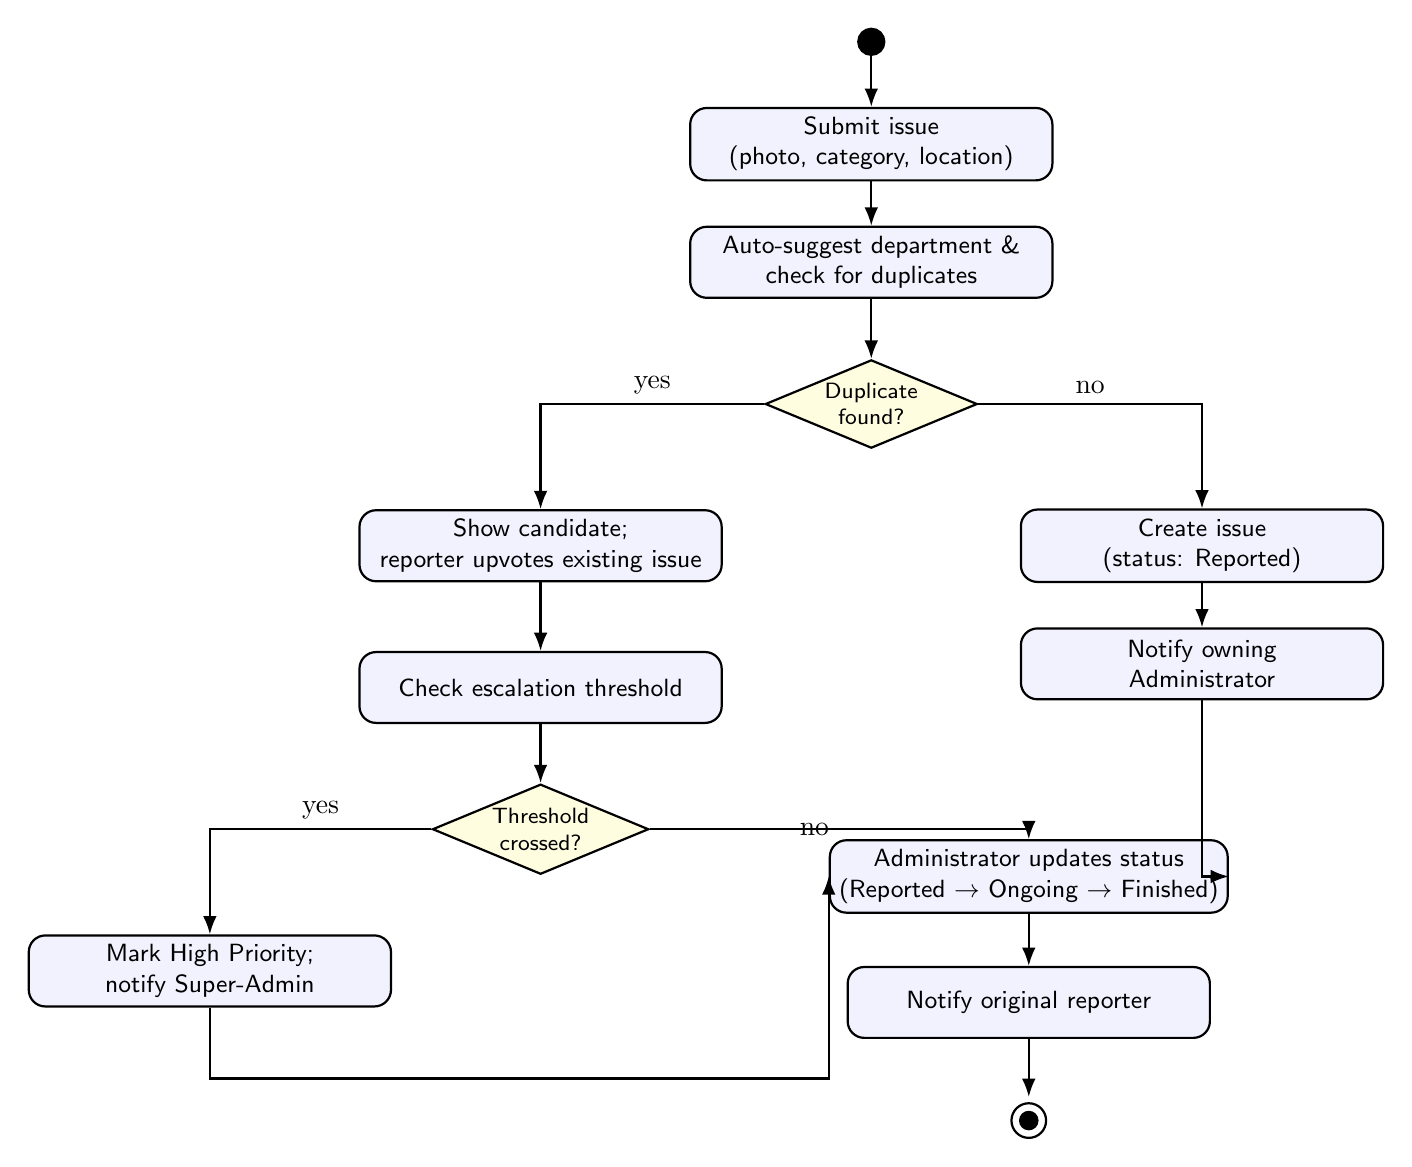
\begin{tikzpicture}[
      action/.style={draw, thick, rounded corners=6pt, minimum width=4.6cm, minimum height=0.9cm, align=center, font=\sffamily\small, fill=blue!5},
      decision/.style={draw, thick, diamond, aspect=2.4, align=center, font=\sffamily\footnotesize, fill=yellow!12, inner sep=1pt},
      startstop/.style={draw, thick, circle, fill=black, minimum size=0.3cm},
      finish/.style={draw, thick, circle, fill=black, minimum size=0.35cm},
      arrowstyle/.style={-Latex, thick}
    ]
    \node[startstop] (start) at (0,15) {};
    \node[action] (submit) at (0,13.7) {Submit issue\\(photo, category, location)};
    \node[action] (suggest) at (0,12.2) {Auto-suggest department \&\\check for duplicates};
    \node[decision] (dupdec) at (0,10.4) {Duplicate\\found?};
    \node[action] (upvote) at (-4.2,8.6) {Show candidate;\\reporter upvotes existing issue};
    \node[action] (create) at (4.2,8.6) {Create issue\\(status: Reported)};
    \node[action] (notifyadmin) at (4.2,7.1) {Notify owning\\Administrator};
    \node[action] (checkesc) at (-4.2,6.8) {Check escalation threshold};
    \node[decision] (escdec) at (-4.2,5.0) {Threshold\\crossed?};
    \node[action] (escalate) at (-8.4,3.2) {Mark High Priority;\\notify Super-Admin};
    \node[action] (updatestatus) at (2,4.4) {Administrator updates status\\(Reported $\to$ Ongoing $\to$ Finished)};
    \node[action] (notifyreporter) at (2,2.8) {Notify original reporter};
    \node[finish] (end) at (2,1.3) {};
    \node[draw, thick, circle, fill=black, inner sep=2pt] () at (2,1.3) {};
    \draw[draw, thick, circle, fill=white] (2,1.3) circle (0.22cm);
    \draw[draw, thick, circle, fill=black] (2,1.3) circle (0.11cm);

    \draw[arrowstyle] (start) -- (submit);
    \draw[arrowstyle] (submit) -- (suggest);
    \draw[arrowstyle] (suggest) -- (dupdec);
    \draw[arrowstyle] (dupdec) -| node[near start, above]{yes} (upvote);
    \draw[arrowstyle] (dupdec) -| node[near start, above]{no} (create);
    \draw[arrowstyle] (create) -- (notifyadmin);
    \draw[arrowstyle] (upvote) -- (checkesc);
    \draw[arrowstyle] (checkesc) -- (escdec);
    \draw[arrowstyle] (escdec) -| node[near start, above]{yes} (escalate);
    \draw[arrowstyle] (escdec) -| node[near start, left]{no} (updatestatus);
    \draw[arrowstyle] (notifyadmin) |- (updatestatus);
    \draw[arrowstyle] (escalate.south) -- ++(0,-0.9) -| (updatestatus.west);
    \draw[arrowstyle] (updatestatus) -- (notifyreporter);
    \draw[arrowstyle] (notifyreporter) -- (2,1.6);
  \end{tikzpicture}}
  \caption{UML activity diagram for the core issue reporting and resolution workflow.}
  \label{fig:activity}
\end{figure}

\section{Implementation Details}

\subsection{Module 1: Reporting and Duplicate Detection}

The submission module implements a structured reporting form: photo
upload, category selection with an automatic department suggestion
(manually overridable by the reporter or an admin), and location entry
via a \emph{Building $\rightarrow$ Floor $\rightarrow$ Area/Room}
hierarchy (dropdowns plus free text), rather than GPS or a map pin,
since GPS is unreliable indoors and map APIs add cost and complexity the
MVP does not need.

Duplicate detection is a heuristic combining three signals, in the
spirit of duplicate bug-report detection studied in the software
engineering literature~\cite{brownlee2006duplicate}, so that no
single weak signal can produce a false match on its own:
\begin{enumerate}
  \item \textbf{Location match} -- exact match on building and floor,
    fuzzy match on the free-text area/room field.
  \item \textbf{Department/category match} -- the new report is only
    compared against issues already routed to the same department.
  \item \textbf{Description similarity} -- a token-overlap / TF-IDF
    cosine similarity measure, with a threshold, between the new
    description and existing open descriptions within the matched
    location/department bucket.
\end{enumerate}
The comparison set is restricted to issues still open (not
\texttt{Finished}), since a resolved issue recurring is a \emph{new}
problem worth a fresh report rather than a duplicate. The system
surfaces the top candidate to the reporter for a human decision and
never fully auto-merges, auto-deletes, or auto-rejects a submission,
keeping a human in the loop for a step that directly affects data
quality.

\textbf{Mid-semester status.} The schema-level support for this module
is in place: a dedicated \texttt{duplicate\_checks} table exists,
along with the description, location, and department fields needed to
run the three-signal match described above. The similarity-matching
logic itself (NLP/TF-IDF comparison) has not been implemented yet, so
at this checkpoint every submission simply creates a new issue; wiring
the matching logic to this schema is scoped as post-mid-semester work
(Section~\ref{sec:mst-scope}).

\subsection{Module 2: Roles, Escalation, and Notifications}

Access is role-based, implemented via JWT-based sessions~\cite{jwt2015}
with role-based access control enforced at the API layer, matching the class
hierarchy of Figure~\ref{fig:classdiagram}. Students and faculty share
identical permissions (report, view all, upvote); Administrators are
scoped to a single department and move issues through their status
lifecycle; the Super-Admin has full cross-department visibility and is
additionally the only role notified on every escalation event
regardless of which department owns the issue. This module -- roles and
status transitions -- is functionally complete and tested (see
Table~\ref{tab:roles} in Chapter~3).

A single flat upvote threshold across every category would either be
too high for safety-critical issues (which should not have to wait for
popularity to earn attention) or too low for high-traffic areas (where
``High Priority'' would stop meaning anything). The design therefore
makes the threshold configurable per category by the Super-Admin, with
a \textbf{default of 5 upvotes} used uniformly for the MVP, since no
real usage data from TIET yet exists to calibrate per-category values
responsibly. This is treated as a known, temporary simplification, to
be reviewed and tuned per category after the pilot.

\textbf{Mid-semester status.} The \texttt{priority} field on
\texttt{Issue} and the per-category \texttt{escalationThreshold} field
on \texttt{Department} (Figure~\ref{fig:classdiagram}) already exist in
the database, but the application logic that checks accumulated upvote
counts against the threshold and flips an issue's priority has not been
written yet -- this is scoped as post-mid-semester work.

Four notification types are designed to close the feedback loop
described in Section~\ref{sec:notifications}, to be delivered via
in-app polling rather than WebSockets to keep the MVP's infrastructure
and failure modes simple. \textbf{Mid-semester status:} the
\texttt{notifications} table and its schema are in place and can be
written to, but the polling mechanism that would surface these
notifications to a user in the UI has not been built yet; this is also
scoped as post-mid-semester work.

\section{Mid-Semester Scope}
\label{sec:mst-scope}

To keep the mid-semester submission honest about what has actually been
built versus what is merely designed, this section states explicitly
which parts of Chapter~2's design are implemented end-to-end today and
which are deliberately deferred to the second half of the project. The
guiding principle has been \emph{schema-first, logic-second}: the
relational schema for every MVP feature was designed and migrated
early (Weeks 1--2 of the timeline) so that the remaining application
logic could be built incrementally against a stable data model, rather
than the schema and logic being developed in lockstep feature-by-feature.

\begin{itemize}
  \item \textbf{Duplicate detection:} the \texttt{duplicate\_checks}
    table and the description/location/department matching structure
    exist in the schema, but the similarity-matching logic (NLP/TF-IDF)
    is not yet built. Every submission currently creates a new issue
    unconditionally.
  \item \textbf{Auto-escalation:} the \texttt{priority} field and the
    per-category \texttt{escalationThreshold} field exist in the
    database, but nothing yet automatically checks upvote counts
    against the threshold and flips priority -- that application logic
    is still to be written.
  \item \textbf{Live notification delivery:} the \texttt{notifications}
    table and its write path work, but the polling mechanism that would
    surface these notifications to a user in the UI is not built.
\end{itemize}

These three items are precisely Objectives 3, 4, and 5 from
Section~1.2, and are the team's explicit focus for the post-mid-semester
phase of the timeline (Weeks 9 onward), alongside the campus pilot in
Section~\ref{sec:pilot}. Everything else described in this
chapter -- the three-tier architecture, the role-based access model, the
structured submission flow, and department routing -- is implemented
and already reflected in the status table in Chapter~3
(Table~\ref{tab:status}).

% ===================================================================
% CHAPTER 3: RESULTS AND EVALUATION
% ===================================================================
\chapter{Results and Evaluation}

This chapter reports progress against the Chapter~2 design as of the
mid-semester checkpoint (end of Week 8 in the project timeline: planning,
authentication/RBAC, the submission-to-database flow, the
duplicate-detection prototype, and the role-scoped dashboards). Since the
campus pilot described in Section~\ref{sec:pilot} runs later in the
schedule, the metrics below distinguish between measurements already
possible on the implemented modules and metrics that are defined and
instrumented but whose real values will only be available once the
pilot generates usage data.

\section{Testing Methodology}

\begin{itemize}
  \item \textbf{Unit testing:} individual backend components -- the
    department-routing function, the duplicate-similarity scorer, and
    the escalation-threshold check -- are tested in isolation with
    fixed input/output cases, run automatically via the CI/CD pipeline
    on every commit.
  \item \textbf{Integration testing:} the submission-to-database flow
    (form $\to$ API $\to$ PostgreSQL $\to$ dashboard) and the
    authentication/RBAC layer are tested end-to-end to confirm that
    each of the four roles can perform exactly its permitted actions
    (Table~\ref{tab:roles}, reproduced from the proposal).
  \item \textbf{Performance testing:} API response time and database
    query time are measured for the duplicate-check and dashboard-list
    endpoints, which are the two most query-heavy code paths.
  \item \textbf{User testing:} a small internal walkthrough with team
    members role-playing Student, Faculty, Administrator, and
    Super-Admin accounts, ahead of the bounded campus pilot.
\end{itemize}

\begin{table}[H]
\centering
\begin{tabular}{@{}lccccl@{}}
  \toprule
  \textbf{Role} & \textbf{Report} & \textbf{View all}
    & \textbf{Upvote} & \textbf{Change status} & \textbf{Scope} \\
  \midrule
  Student        & \checkmark & \checkmark & \checkmark & --         & -- \\
  Faculty        & \checkmark & \checkmark & \checkmark & --         & -- \\
  Administrator  & --         & \checkmark & --         & \checkmark & Own department \\
  Super-Admin    & --         & \checkmark & --         & \checkmark & All departments \\
  \bottomrule
\end{tabular}
\caption{Role-based permission matrix verified by integration tests.}
\label{tab:roles}
\end{table}

\section{Implementation Status}

\begin{table}[H]
\centering
\begin{tabular}{|p{6.4cm}|p{2.6cm}|p{5cm}|}
\hline
\textbf{Feature} & \textbf{Status} & \textbf{Notes} \\
\hline
JWT auth + RBAC (4 roles) & Complete & Verified by integration tests against Table~\ref{tab:roles}. \\
\hline
Structured submission form (photo, category, location) & Complete & Department auto-suggestion implemented; manual override in progress. \\
\hline
Duplicate-detection heuristic & Prototype & Location + department filtering complete; description-similarity threshold under tuning. \\
\hline
Administrator / Super-Admin dashboards & In progress & Read/list views complete; status-transition controls being wired to the API. \\
\hline
Auto-escalation engine & Planned & Scheduled for Week 9 per the project timeline. \\
\hline
Notifications (4 event types, polling) & Planned & Scheduled alongside escalation. \\
\hline
CI/CD pipeline (build, lint, test, staging deploy) & Complete & Runs on every push via GitHub Actions. \\
\hline
\end{tabular}
\caption{Implementation status of MVP deliverables at the mid-semester checkpoint.}
\label{tab:status}
\end{table}

\section{Evaluation Metrics}

The following metrics are defined for the platform, each corresponding
to a specific feature in Chapter~2. Values marked ``pending pilot'' are
instrumented in the schema (e.g. status timestamps, the
\texttt{read\_status} field) but require real reporting volume from the
campus pilot to be meaningful.

\begin{table}[h]
\centering
\begin{tabular}{|p{4.6cm}|p{5.4cm}|p{3.6cm}|}
  \hline
  \textbf{Metric} & \textbf{Definition} & \textbf{Status} \\
  \hline
  Time-to-first-action (TTFA) & Time between an issue entering \texttt{Reported} and its first transition to \texttt{Ongoing} & Pending pilot \\
  \hline
  Duplicate-detection precision & Proportion of surfaced duplicate candidates that reporters accept (upvote) rather than reject & Instrumented; preliminary internal tests show correct flagging on same-location/category test cases \\
  \hline
  Escalation precision & Proportion of auto-escalated issues an Administrator agrees warranted High Priority & Pending pilot (escalation engine not yet live) \\
  \hline
  Resolution time by category & Time from \texttt{Reported} to \texttt{Finished}, by category & Pending pilot \\
  \hline
  Duplicate deflection rate & Proportion of submissions ending as an upvote rather than a new report & Pending pilot \\
  \hline
  Notification effectiveness & Proportion of notifications marked read within a defined window & Pending pilot (notification module not yet live) \\
  \hline
\end{tabular}
\caption{Evaluation metrics and their status at the mid-semester checkpoint.}
\label{tab:performance}
\end{table}

\section{Pilot Validation Plan}
\label{sec:pilot}

Once the remaining MVP modules (escalation, notifications) are
complete, the platform will be validated with a bounded pilot: one or
two hostel blocks plus one academic block, rather than campus-wide, to
keep reporting volume interpretable within the course timeline. A small
set of student/faculty reporters will be recruited, with Administrator
accounts either staffed by real departmental personnel where available
or simulated by the team. An informal baseline -- a short survey on how
long informally-reported issues currently take to get attention -- will
give the metrics in Table~\ref{tab:performance} a comparison point,
since no institutional baseline is tracked today.

\section{Analysis}

Against the six objectives in Section~1.2, Objectives 1, 2, and 6 are
substantially met at this checkpoint: the reporting form, automatic
routing, and role-scoped access are implemented and tested. Objective 3
(duplicate prevention) is partially met -- the heuristic's structural
signals (location, department) work reliably, but the description
similarity threshold needs tuning against a larger and more varied set
of sample descriptions than the team could generate internally, which
is expected and is the reason the pilot exists. Objectives 4 and 5
(escalation and the closed notification loop) are on schedule but not
yet implemented, consistent with the Week 9 target in the project
timeline; no claims about their real-world behaviour can be made before
they are live.

The main challenge encountered so far has been calibrating the
duplicate-similarity threshold without real user-submitted description
data: an overly strict threshold misses genuine duplicates, while an
overly loose one produces false positives that could discourage
legitimate reports. Per the risk mitigation in the original proposal,
the team resolved this by always surfacing the candidate for a human
decision rather than attempting to auto-tune the threshold from
synthetic data, and by treating duplicate-detection precision
(Table~\ref{tab:performance}) as a live signal to revisit once pilot
data exists.

% ===================================================================
% CHAPTER 4: CONCLUSION
% ===================================================================
\chapter{Conclusion}

\section{Summary of Work}

This report has described the design and progressing implementation of
the \sysname, a role-based web platform for reporting, tracking, and
resolving campus infrastructure issues at TIET. Students and faculty can
report problems such as electrical, plumbing, cleanliness, or other
infrastructure issues with a photo, category, and structured location;
department Administrators receive and manage issues routed to their
department; and a Super-Admin provides institution-wide oversight. The
system follows a three-tier architecture (React, Node.js/Express,
PostgreSQL) with object storage for images and JWT-based role-based
access control, as detailed in Chapter~2. At the mid-semester
checkpoint, authentication/RBAC, the structured submission flow, a
duplicate-detection prototype, and CI/CD are complete, with dashboards
in progress and escalation/notifications on schedule for the following
weeks (Table~\ref{tab:status}).

\section{Key Findings}

\begin{itemize}
  \item \textbf{Finding 1:} Restricting duplicate comparison to
    \emph{open} issues within the same location/department bucket
    (rather than the full historical issue table) keeps the check both
    semantically correct -- a resolved issue recurring is a new problem
    -- and cheap, since its cost does not grow with total historical
    volume.
  \item \textbf{Finding 2:} A single flat escalation threshold is a
    reasonable placeholder for an MVP but is explicitly a simplification;
    safety-critical and high-traffic categories genuinely need different
    thresholds, which is only sensible to calibrate once real
    upvote-volume data exists.
  \item \textbf{Finding 3:} Keeping a human in the loop for the
    duplicate decision (upvote vs.\ new report) turned out to be not
    just a safety choice but also the most practical source of a
    trainable precision signal, since it converts every submission into
    a labelled data point without requiring a separate hand-labelling
    effort.
\end{itemize}

\section{Future Work and Recommendations}

\begin{itemize}
  \item Complete the auto-escalation engine and the four-type
    notification service (Week 9 of the timeline).
  \item Replace the flat MVP escalation threshold with per-category
    thresholds calibrated using real pilot upvote-volume data.
  \item Improve duplicate-detection similarity (e.g., embedding-based
    similarity in place of pure token overlap/TF-IDF) once enough real
    description data exists to evaluate it meaningfully.
  \item Add aggregate analytics for facilities management: recurring-issue
    hotspots by building/category and resolution-time trends over time.
  \item Consider an optional email/SMS notification channel alongside
    in-app notifications, and search/filtering improvements on the
    public issue list as report volume grows.
\end{itemize}

\section{Final Remarks}

The project's central engineering bet is that campus issue resolution is
bottlenecked by \emph{visibility and routing}, not maintenance capacity,
and that a structured, trackable reporting channel can address that
bottleneck without requiring any change to how maintenance work itself
is carried out. The mid-semester progress supports this framing: the
hardest design problems so far have been about correctly scoping the
duplicate check and choosing sensible defaults under missing data,
rather than about the underlying three-tier architecture, which has
proceeded largely as planned. The remaining work -- escalation,
notifications, and the campus pilot -- is what will determine whether
the system's routing, duplicate handling, and prioritization actually
improve outcomes in practice, and the evaluation plan in
Section~\ref{sec:pilot} has been designed specifically to make that
determination measurable rather than anecdotal.

% ===================================================================
% BIBLIOGRAPHY (plain thebibliography -- no biber/references.bib needed)
% ===================================================================
\begin{thebibliography}{9}

\bibitem{sommerville2016}
I.~Sommerville, \emph{Software Engineering}, 10th ed. Pearson, 2016.

\bibitem{fielding2000rest}
R.~T.~Fielding, ``Architectural Styles and the Design of Network-based
Software Architectures,'' Ph.D. dissertation, Univ. of California,
Irvine, 2000.

\bibitem{postgresql2024}
The PostgreSQL Global Development Group, \emph{PostgreSQL Documentation},
2024.

\bibitem{fowler2004uml}
M.~Fowler, \emph{UML Distilled: A Brief Guide to the Standard Object
Modeling Language}, 3rd ed. Addison-Wesley, 2004.

\bibitem{elmasri2015}
R.~Elmasri and S.~B.~Navathe, \emph{Fundamentals of Database Systems},
7th ed. Pearson, 2015.

\bibitem{jwt2015}
M.~Jones, J.~Bradley, and N.~Sakimura, ``JSON Web Token (JWT),'' RFC 7519,
IETF, 2015.

\bibitem{brownlee2006duplicate}
N.~Bettenburg, S.~Just, A.~Schr\"oter, C.~Weiss, R.~Premraj, and
T.~Zimmermann, ``Duplicate Bug Reports Considered Harmful \dots Really?,''
in \emph{Proc. IEEE Int. Conf. Software Maintenance (ICSM)}, 2008.

\end{thebibliography}

\end{document}
